\documentclass[%
 reprint,
%superscriptaddress,
%groupedaddress,
%unsortedaddress,
%runinaddress,
%frontmatterverbose, 
%preprint,
%preprintnumbers,
%nofootinbib,
%nobibnotes,
%bibnotes,
% aapm,
amsmath,
amssymb,
%%%% amsthm,amssymb,mathtools,mathpazo,physics
%  mph,
%  aps,
% pra,
% prb,
% rmp,
%prstab,
%prstper,
%floatfix,
10pt
]{revtex4-2}

\usepackage{graphicx}% Include figure files
\usepackage{dcolumn}% Align table columns on decimal point
\usepackage{bm}% bold math
\usepackage[colorlinks]{hyperref}% add hypertext capabilities
\usepackage{multirow}
%\usepackage[mathlines]{lineno}% Enable numbering of text and display math
%\linenumbers\relax % Commence numbering lines

%\usepackage[showframe,%Uncomment any one of the following lines to test 
%%scale=0.7, marginratio={1:1, 2:3}, ignoreall,% default settings
%%text={7in,10in},centering,
%%margin=1.5in,
%%total={6.5in,8.75in}, top=1.2in, left=0.9in, includefoot,
%%height=10in,a5paper,hmargin={3cm,0.8in},
%]{geometry}
% \usepackage{subfig}
\usepackage[%
    font={small,sf},
    labelfont=bf,
    format=hang,    
    format=plain,
    margin=0pt,
    width=0.8\textwidth,
]{caption}
\usepackage[list=true]{subcaption}
\usepackage{float}
% \usepackage{pdfpages}
% \usepackage{pgffor}

% \makeatletter
% \AtBeginDocument{\let\LS@rot\@undefined}
% \makeatother

\renewcommand{\arraystretch}{1.2}
\newcommand{\bs}[1]{\boldsymbol{#1}}
\newcommand{\dd}[1]{\mathrm{d}{#1}}

\begin{document}

% \preprint{APS/123-QED}

\title{P443 \& P444: Study of Non-Linear Optical Properties using Z-Scan}% Force line breaks with \\

\author{Jyotirmaya Shivottam}
\email{jyotirmaya.shivottam@niser.ac.in}
\affiliation{%
 National Institute of Science Education and Research, Bhubaneswar, India
}%

\date{\today}

\begin{abstract}
In this experiment, we have explored the Single Beam Z-Scan Technique put forward by Sheikh-Bahae et al \cite{bahae} and obtained Z-Scan traces for these materials: \textit{SKK1}, \textit{SKK2} and \textit{Nanorods} on \textit{Tempered Glass} and \textit{Standard Glass} substrates. We have analyzed these traces using Python and calculated the Non-Linear Refractive Index ($n_2$) and the Non-Linear Absorption Coefficient ($\beta$) for all the materials. We have also examined certain future directions that one could take this experiment in.
\end{abstract}

\keywords{z-scan, non-linear optics, non-linear refractive index, non-linear absorption coefficient, saturable absorption}%Use showkeys class option if keyword

\maketitle

\tableofcontents

\section{\label{intro}Introduction}
\subsection{\label{overview}Overview}
\begin{figure*}
    \centering
    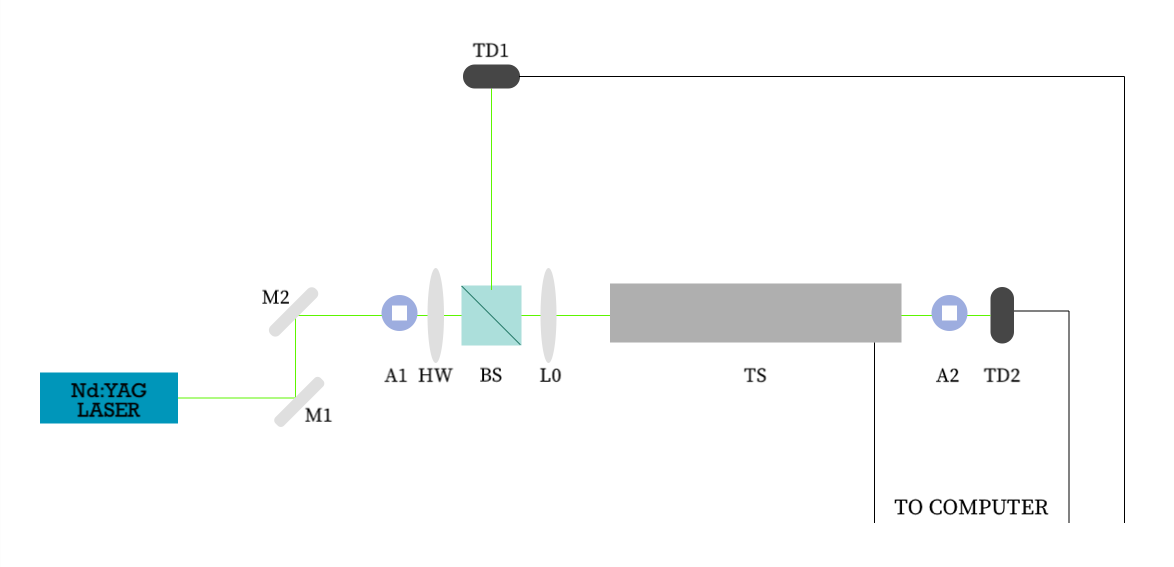
\includegraphics[width=0.65\textwidth]{images/schem.png}
    \caption{Schematic of the Experimental Setup. Please consult Subsection - \ref{setup} to follow the acronyms used here.}
    \label{fig:schem}
\end{figure*}

\begin{figure}
\subcaptionbox{Non-Linear Refraction}{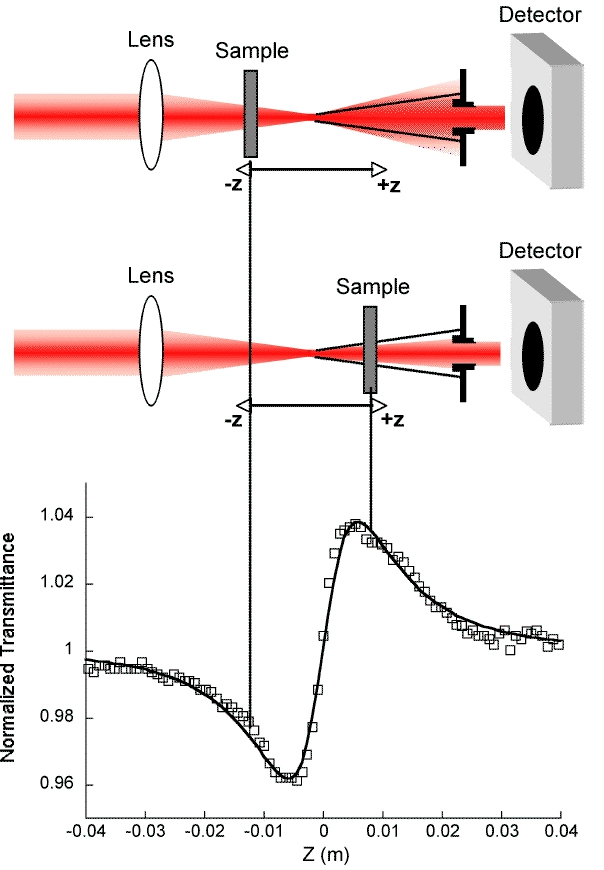
\includegraphics[width=0.34\textwidth]{images/thca.jpg}}\\%
\subcaptionbox{Non-Linear Absorption}{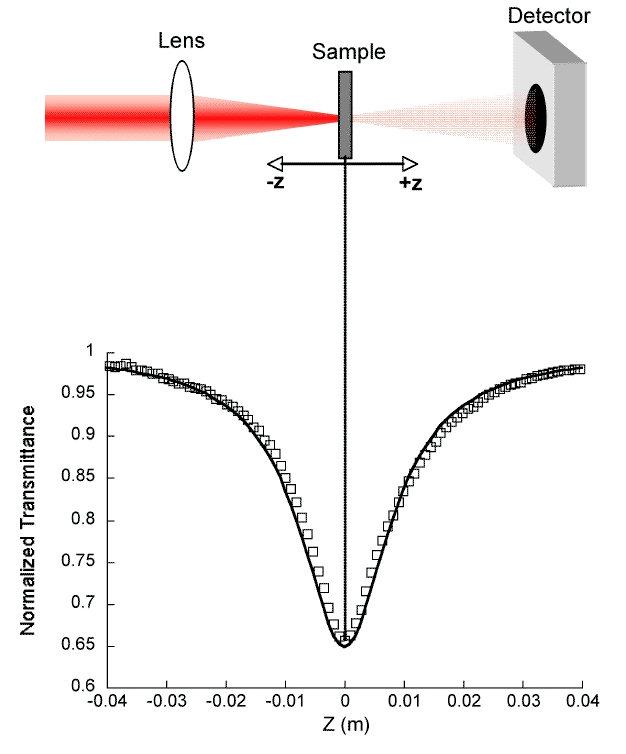
\includegraphics[width=0.38\textwidth]{images/thoa.jpg}}%
\captionsetup{width=0.4\textwidth}
\caption{Z-Scan Traces highlighting non-linear optical properties [\href{http://cleanenergywiki.org/index.php?title=Femtosecond_Z-Scan_Spectrometer}{Source}]}
\label{fig:th2}
\end{figure}

\begin{figure}
    \centering
    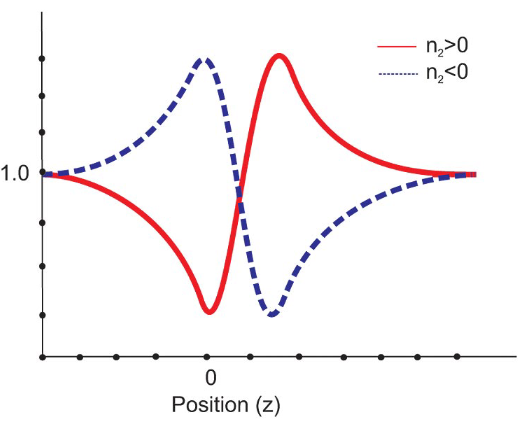
\includegraphics[width=\linewidth]{images/swap.png}
    \caption{Swapping of peak and valley, with change in sign [\href{https://www.holmarc.com/z_scan_system.php}{Source}]}
    \label{fig:swap}
\end{figure}

The non-linear optical properties of materials have found several applications in recent times, primarily in ultra-fast optical switching and signal processing applications. In such cases, the relevant phenomena are Non-Linear Refraction (NLR) and Non-Linear Absorption (NLA). The Single Beam Z-Scan technique, devised by Sheikh-Bahae et al \cite{bahae}, is one of the principal techniques to explore these non-linear material characteristics owing to its simplicity and high sensitivity. This technique can rapidly provide a measure of both NLR and NLA in solids as well as liquids (including solutions), yielding the sign as well as the magnitude of the non-linear refractive index ($n_2$) and the non-linear absorption coefficient ($\beta$). This technique is based on the principles of spatial beam distortion. It makes use of the fact that a spatially transverse variation in LASER intensity induces non-linear optical changes in the material, giving rise to a lens-like effect, which in turn affects the beam propagation. This leads to a self-focusing or defocusing effect (self-lensing effect) as can be seen in Fig.~\ref{fig:th2}. This in turn causes changes in the far-field diffraction pattern, that can be utilized to obtain the relevant non-linear optical properties of materials. ``Single Beam", in the name, comes from the fact that a single Gaussian laser beam in a tight focus geometry (as shown in Fig.~\ref{fig:schem}), is used to induce the non-linear effects.\\

In this technique, high intensity LASER light is shined on a non-linear medium and then the on-axis intensity of the far-field diffraction pattern, through a finite aperture is considered. In particular, we examine the behaviour of Normalized Transmittance ($T(z)$), as a function of the sample position ($z$), that is measured with respect to the focal point of the converging lens. To further clarify the relationship between the Z-Scan trace and the non-linear optical properties ($n_2$ and $\beta$), consider Fig.~\ref{fig:th2}. Here, for a material with positive $n_2$ and negligible NLA, and a thickness lesser than the Rayleigh length of the focused beam, we can think of the sample as a thin lens of variable focal length. Starting at negative $z$ (with respect to $L0$'s focus, Fig.~\ref{fig:schem}), the beam intensity is low and minimal nonlinear refraction takes place, which leads to a relatively constant transmittance value. As the sample moves closer to the focus, the beam intensifies, resulting in self-lensing in the material. A positive self-lensing effect tends to diverge the beam, effecting beam-widening at the aperture, that causes a drop in the transmittance value. On the other side of the focus, the same effect tends to collimate the beam, causing an increase in the transmittance value. This also implies that $T(z)$ has a null at $L0$'s focus, which is analogous to the little to no change in far-field diffraction pattern, caused by placing a thin lens at the focus. Again, further beyond the focus, the transmittance becomes nearly constant, since the beam intensity drops. For a material with a positive $\beta$ value and negligible NLR, the Z-Scan trace has a similar explanation. The absorbance of the material is nearly constant at points, far away from the focus, but it increases, as the sample moves closer to the focus, leading to a drop in transmittance, whereas it decreases as the sample moves away from the focus, causing the transmittance to recover to a nearly constant value, as can be seen in Fig.~\ref{fig:th2}. A noteworthy point is that the location of peaks and valleys in the traces swap, if the material has a negative $n_2$ or a negative $\beta$ value, as shown in Fig.~\ref{fig:swap}. A good resource to actively visualize these changes is \href{http://www.phys.unm.edu/msbahae/z-scan.htm}{this animated tool}.\\

In this experiment, we have investigated the Z-Scan technique with 4 samples, two of which are organic solutions, while two are Nanorod wafers on 2 different substrates. In particular, we have taken Closed (CA) and Open (OA) Aperture Z-Scan traces for all the samples and analyzed them with Python code, in order to calculate the non-linear refractive index ($n_2$) and the non-linear absorption coefficient ($\beta$) values for all samples. We have also constrained these values with error analysis and interpreted the traces.\\

In the next subsection, we expand on the theory of Z-Scan and briefly explore the effect of aperture on the traces. Then, in Section - \ref{meth}, we detail the apparatus and procedure for this experiment and in Section - \ref{obs}, we present our observations. Ultimately, in Section - \ref{dis}, we discuss our results as well as the experimental setup. We have also presented some extensions to this experiment in the same section. Due to large plots, we have placed all the Z-Scan traces in an appendix, that can be found near the end of this document.

\subsection{\label{th}Theory}
Consider a Gaussian Beam, propagating along the $z-$direction with beam waist, $w_0$, wavelength, $\lambda$, and Rayleigh Length, $z_0 = \pi w_0^2 / \lambda$:
\begin{widetext}
\begin{equation}
    \boxed{
    E(r, z) = E_0(t)\frac{w_0}{w(z)}\exp{\left(-\frac{r^2}{w(z)^2}\right)}\exp{\left(-ikz -ik\frac{r^2}{2R(z)}\right)}\exp(-i\phi(z,t))
    }.
    \label{eq:E}
\end{equation}
\end{widetext}
Here, $k = 2\pi / \lambda$ is the Wave Number; $w(z) = w_0(1 + x^2)$ represents the Beam Width, with $x = z / z_0$; and $R(z) = z(1 + x^2)$ denotes the Radius of Curvature. The last term, $\exp(-i\phi(z,t))$, contains all the radially uniform phase variations. As we only wish to obtain the radial phase variations, $\Delta\phi(r)$, we can apply the Slowly Varying Envelope Approximation (SVEA) and ignore phase changes that are uniform in $r$. Now, let this beam be transmitted through a Kerr non-linear optical material of length, $L$. Then, considering a centrosymmetric medium, we can write the refractive index and absorption coefficient as:
\begin{equation}
    n(I) = n_0 + n_2 I,
    \label{eq:n}
\end{equation}
\begin{equation}
    \alpha(I) = \alpha_0 + \beta I;
    \label{eq:alpha}
\end{equation}
where, $n_0$ is the linear refractive index, while $n_2$ denotes the non-linear refractive index and $\alpha_0$ is the linear absorption coefficient, while $\beta$ represents the non-linear absorption coefficient. $I$ denotes the intensity of light. For a thin sample, the output field can be written as follows:
\begin{equation}
    E_{out} = E(r, z)e^{-\frac{\alpha_0 L}{2}}(1 + q)^{-\frac{ikn_2}{\beta} - \frac{1}{2}},
    \label{eq:Eout1}
\end{equation}
where, $q = \beta I L_{eff}$ with $L_{eff} = (1 - e^{-\alpha_0 L}) / \alpha_0$, and $I_0 = |E_0|^2$ is the on-axis intensity at beam waist. For very thin samples, such as in this experiment, we can take $L_{eff} \approx 1$ (in proper units). Moreover, $I_0$ can be written as:
\begin{equation}
    I_0 = \frac{P_{Avg}}{RR\times PW\times(\pi w_0^2)},
    \label{eq:I0}
\end{equation}
where, $P_{Avg}$ is the average beam power, $RR$ is the LASER Repetition Rate, $PW$ is the LASER Pulse Width and $\pi w_0^2$ is the beam area, at focus.\\

The intensity distribution and phase shift of the beam, at the exiting surface, must also fulfill these criteria \cite{calc}:
\begin{equation}
    I_{out}(r, z) = I(r, z)\frac{\exp(-\alpha_0 L)}{1 + q(r, z)},
    \label{eq:IOut}
\end{equation}
and,
\begin{equation}
    \Delta\phi = \frac{kn_2}{\beta}\ln(1 + q(r, z)).
    \label{eq:delphi}
\end{equation}
Now, the intensity, $I(r, z)$, can be expressed as the product of $I_0$ and a local Gaussian profile, $G_{local}$ \cite{calc}, that can be written as follows:
\begin{equation}
    G_{local} = \frac{1}{1 + x^2}\exp\left(-\frac{2r^2}{w^2(z)}\right).
    \label{eq:GLoc}
\end{equation}
When only NLR is present, we can write the non-linear phase change as:
\begin{equation}
    \Delta\phi = \Delta\Phi_0 G_{local},
    \label{eq:delphi2}
\end{equation}
while for materials exhibiting pure NLA, $q$ takes the following form:
\begin{equation}
    q(r) = \Delta\Psi_0 G_{local},
    \label{eq:qq}
\end{equation}
Here, $\Delta\Phi_0$ and $\Delta\Psi_0$ are merely the results of the respective first order expansions of the expressions for $\Delta\phi$ (Eq.~\ref{eq:delphi}) and $q$, in the cases of pure NLR and pure NLA respectively. This gives us:
\begin{equation}
    \boxed{\Delta\Phi_0 = kn_2 I_0 L_{eff}},
    \label{eq:deltaphi}
\end{equation}
and,
\begin{equation}
    \boxed{\Delta\Psi_0 = 2^{-1.5}\beta I_0 L_{eff}}.
    \label{eq:deltapsi}
\end{equation}

Substituting these quantities from Eq.~\ref{eq:delphi2} and Eq.~\ref{eq:qq} into Eq.~\ref{eq:Eout1}, we obtain a final expression for the outgoing field:
\begin{equation}
    E_{out} = E(r, z)e^{-\frac{\alpha_0 L}{2}}(1 + \Delta\Psi_0 G_{local})^{-\frac{i\Delta\Phi_0}{\Delta\Psi_0} - \frac{1}{2}}.
    \label{eq:EFinal}
\end{equation}

Now, making use of SVEA and the Gaussian Decomposition method for local field changes and considering only the first two terms in the decomposition, we can obtain an analytical expression for the complex, on-axis far-field given as (\cite{bahae}, \cite{calc}):
\begin{widetext}
\begin{equation}
    \boxed{
    E_{out} = E(r, z)\exp\left(-\frac{\alpha_0 L}{2}\right)  \sum_{n = 0}^\infty\left[ \frac{[-i\Delta\phi_0(z)]^n}{n!} \prod_{n' = 0}^{n}\left(1 - i(2n' - 1)\frac{\Delta\Psi_0}{\Delta\Phi_0}\right)\right] \exp\left(\frac{-2nr^2}{w^2(z)}\right)
    }.
    \label{eq:Eout2}
\end{equation}
\end{widetext}

Using Eq.~\ref{eq:Eout2}, we can write the complex field at the aperture plane, as follows:
\begin{widetext}
\begin{equation}
    \boxed{
    E_a = E(r, z)\sum_{n = 0}^\infty \frac{[-i\Delta\phi_0(z)]^n}{n!} \prod_{n' = 0}^{n}\left(1 - i(2n - 1)\frac{\Delta\Psi_0}{\Delta\Phi_0}\right)\frac{w_{n0}}{w_n}\exp\left(-\frac{r^2}{w_n^2} - \frac{ikr^2}{2R_n} + i \theta_n\right)
    }.
    \label{eq:Ea}
\end{equation}
\end{widetext}
Here, $\Delta\phi_0 = \Delta\Phi_0 / (1 + x^2)$.\\

When only NLR is considered, $\Delta\Psi_0 \to 0$, and we can reduce the previous equation to obtain:
\begin{widetext}
\begin{equation}
    \boxed{
    E_a = E(r, z)\sum_{n = 0}^\infty \frac{[-i\Delta\phi_0(z)]^n}{n!}\frac{w_{n0}}{w_n}\exp\left(-\frac{r^2}{w_n^2} - \frac{ikr^2}{2R_n} + i \theta_n\right)
    }.
    \label{eq:Ea2}
\end{equation}
\end{widetext}
Taking $d$ to be the propagation distance in free space, between the sample and the aperture, and $g = 1 + d / R(z)$, we can represent the parameters in Eq.~\ref{eq:Ea} and \ref{eq:Ea2} as follows:
\begin{equation*}
    w_{n0}^2 = \frac{w^2(z)}{2n + 1},
    \label{eq:wn0}
\end{equation*}

\begin{equation*}
    d_n = \frac{kw_{n0}^2}{2},
    \label{eq:dn}
\end{equation*}

\begin{equation*}
    w_n^2 = w_{n0}^2\left(g^2 + \frac{d^2}{d_n^2}\right),
    \label{eq:wn}
\end{equation*}

\begin{equation*}
    R_n^2 = d\left(1 - \frac{g}{g^2 + d^2 / d_n^2}\right)^{-1},
    \label{eq:Rn}
\end{equation*}

and,
\begin{equation*}
    \theta_n = \tan^{-1}\left(\frac{d}{g d_n}\right).
    \label{eq:thetan}
\end{equation*}

The total transmitted power through the aperture can then be obtained by spatially integrating $E_a(r, t)$, like so:
\begin{equation}
    P_T(\Delta\Phi_0(t)) = \int_0^{r_{a}}|E_a(r, t)|^2 r \mathrm{d}r .
    \label{eq:PT}
\end{equation}
This directly yields the normalized Z-Scan transmittance, $T(z)$, using the following expression:
\begin{equation}
    T(z) =  \frac{\int_{-\infty}^\infty P_T(\Delta\Phi_0(t))\mathrm{d}t}{S\int_{-\infty}^\infty P_i(t) \mathrm{d}t},
    \label{eq:Tz}
\end{equation}
where $P_i(t) = \pi w_0^2 I_0(t) / 2$ is the instantaneous input power, within the sample, and $S = 1 - \exp(-2r_a^2/w_a^2)$, where subscript - $a$ denotes ``aperture". This is where the aperture-dependence of the Z-Scan traces comes in. For closed aperture traces, we can take $S \approx 0$ and for open aperture traces, $S \approx 1$. Now, the normalized transmittance for the on-axis electric field, at the aperture plane, can be written as:
\begin{equation}
    \boxed{
        T_2(z, \Delta\phi_0) = \frac{|E(r=0,z,\Delta\phi_0|^2}{|E(r=0,z,\Delta\phi_0 = 0|^2}
    }.
    \label{eq:T2}
\end{equation}
On substituting the expression for the field into Eq.~\ref{eq:T2} and simplifying, we obtain the final expression for $T(z)$, that considers the effect of both NLR and NLA, as given below:
\begin{widetext}
\begin{equation}
    \boxed{
        T_2(z, \Delta\Phi_0, \Delta\Psi_0) = 1 + \frac{4\Delta\Phi_0 x}{(x^2 + 9)(x^2 + 1)}  - \frac{\Delta\Psi_0}{x^2 + 1}
    }.
    \label{eq:T22}
\end{equation}
\end{widetext}
Eq.~\ref{eq:T22} provides a two-parameter fitting function for any third-order Z-Scan trace, the two parameters being $\Delta\Phi_0$ and $\Delta\Psi_0$, and we have used it to fit the closed aperture traces, in order to obtain the $n_2$ values in this experiment. On the other hand, for $\beta$ values, we take the open aperture traces, that de-emphasize $\Delta\Phi_0$ or small intensity variations, as the entire signal is being measured. So, we can provide a simpler, one-parameter expression for $T(z)$ in this case:
\begin{equation}
    \boxed{
        T_2(z, \Delta\Phi_0 = 0, \Delta\Psi_0) = 1  - \frac{\Delta\Psi_0}{x^2 + 1}
    }.
    \label{eq:T2o}
\end{equation}

\begin{figure}
\subcaptionbox{Case 1: Pure Non-Linear Refraction. Note the symmetric peak and valley. (NLR)}{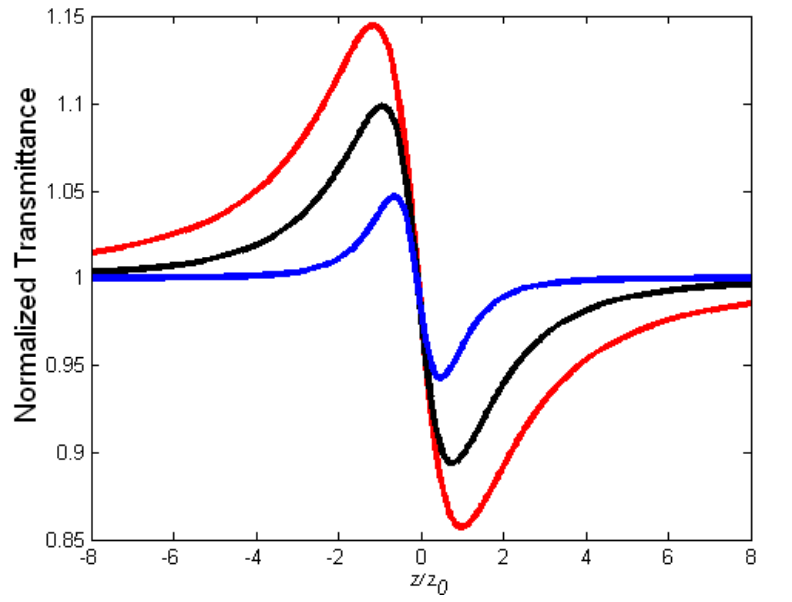
\includegraphics[width=\linewidth]{images/thcapic.png}}\\%
\subcaptionbox{Case 2: Pure Non-Linear Absorption (NLA)}{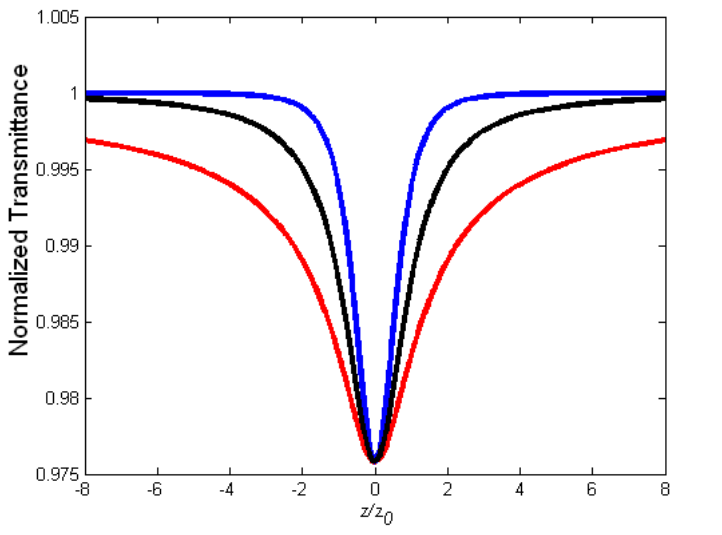
\includegraphics[width=1.03\linewidth]{images/thoapic.png}}\\%
\subcaptionbox{Case 3: Mixed case. NLA suppresses NLR, leading to a skewed trace.}{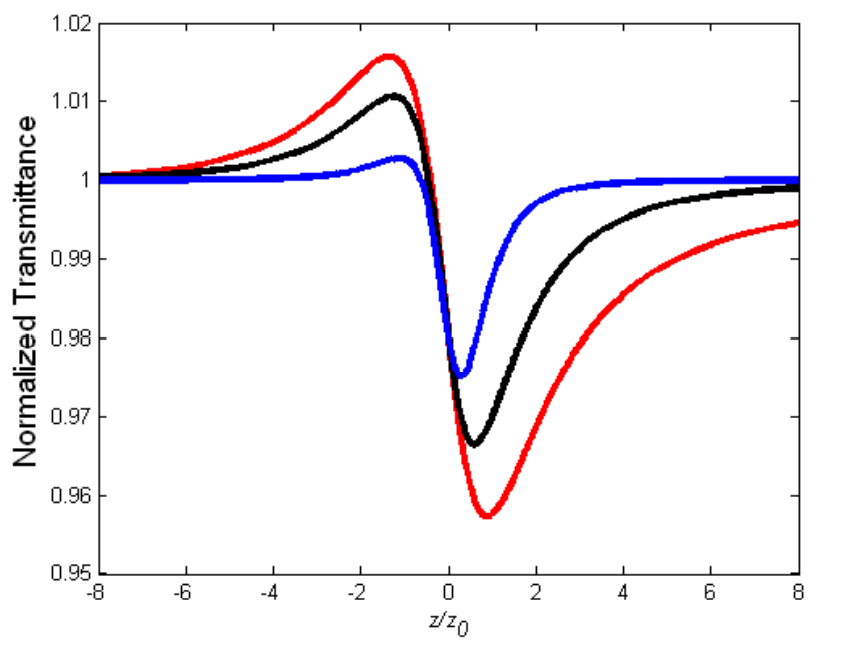
\includegraphics[width=\linewidth]{images/thall.png}}%
\caption{Some plots based on Eq.~\ref{eq:T22} \cite{calc}}
\label{fig:Tvar}
\end{figure}

Equations~\ref{eq:T22} and \ref{eq:T2o} are the working formulae for this experiment. Figure~\ref{fig:Tvar} shows variations in transmittance in Z-scan traces for materials exhibiting pure NLR, pure NLA and both NLR and NLA (mixed case), using various values for $\Delta\Phi_0$ and $\Delta\Psi_0$. It is clear from the plots that NLA suppresses peaks in the mixed Z-Scan traces, as compared to the pure NLR case. This also means that the symmetric nature of pure NLR curves is usually absent in most Z-Scan traces, where both NLR and NLA contribute. As such, we can utilize another interesting quantity, that is the \textit{Peak-Valley Transmittance Change}, $\Delta T_{p-v}$. It is expressed as follows in the closed aperture case (where we shall be using the two-parameter fitting function in Eq.~\ref{eq:T22}):
\begin{equation}
    \boxed{
        \Delta T_{p-v} = 0.406\Delta\Phi_0
    }.
    \label{eq:Tpv}
\end{equation}
This relation for $\Delta T_{p-v}$ should hold even for highly skewed Z-Scan traces. Therefore, it provides us with an excellent tool to verify the quality of our traces.

\section{\label{meth}Methodology}
\subsection{\label{setup}Experimental Setup}
We have made use of the following equipment for this experiment:
\begin{enumerate}
    \item The main setup:
    \begin{enumerate}
        \item A $532\:nm$ $Q-$Switched Nd:YAG LASER operating at $80\:KHz$ Repetition Rate for alignment and measurement of beam waist, and at $1\:KHz$ or $8\:KHz$ for taking measurements. The Pulse Width of the LASER is $1.75\:ns$.
        \item Two reflecting mirrors (M1 \& M2), placed in Z-Fold configuration as shown in \ref{fig:schem}, to save space and to easily align the setup.
        \item A Half-Wave (HW) plate to control the intensity of the LASER light, falling on the sample.
        \item A Beam Splitter (BS) to both control light intensity, as well as to divert the light to a detector to check for intensity fluctuations.
        \item 2 Adjustable Pin-Hole Apertures (A1 \& A2). A1 is used to control the light intensity, while A2 is used to to perform the Z-Scan with variable aperture sizes. They also help in aligning the LASER.
        \item A Converging Lens (L0), with $f = 15\:cm$, to focus the LASER light.
        \item 2 Thermal Detectors (TD1 \& TD2) with up to micro-watt resolution, along with cables to connect to a Computer.
        \item A Translation Stage (TS) with wires and control software. It has a stepper motor, which can run at up to $300$ RPM. The end-to-end length covered by the translation stage, with the mounted sample, is $12.2\:cm$ ($\approx 12400$ steps).
        \item A Beam Profiler to measure the Beam Waist.
        \item An Optical Table to assemble the setup.
        \item StarLab software and a computer to take the readings.
        \item Allen Keys and bolts to hold the equipment in place.
        \item Multiple screens to avoid interference from other setups.
    \end{enumerate}
    \item For handling \& labeling samples
    \begin{enumerate}
        \item $5\:ml$ Dropper
        \item Gloves
        \item Scissors
        \item Tissue Paper
        \item Cuvettes ($1\:ml$), with length of axial (thin) side $=1\:mm$, to hold the liquid samples
        \item Small Corner Bracket to hold the solid samples
        \item Organic solutions (Acetone, DMSO) to clean the cuvettes
        \item Double-sided Tape to hold samples in place
        \item Permanent Marker or Pen to label samples, as well as to mark lengths
    \end{enumerate}
    \item Some additional equipment, that also proved useful:
    \begin{enumerate}
        \item Measuring tape or ruler to measure distances
        \item Small card, e.g. a business card, that can be used to follow and view the LASER beam at any location along the setup
        \item Weighing Scale (Least count $\approx 10\:mu g$) to measure mass of the organic samples
    \end{enumerate}
\end{enumerate}

\begin{figure}
    \centering
    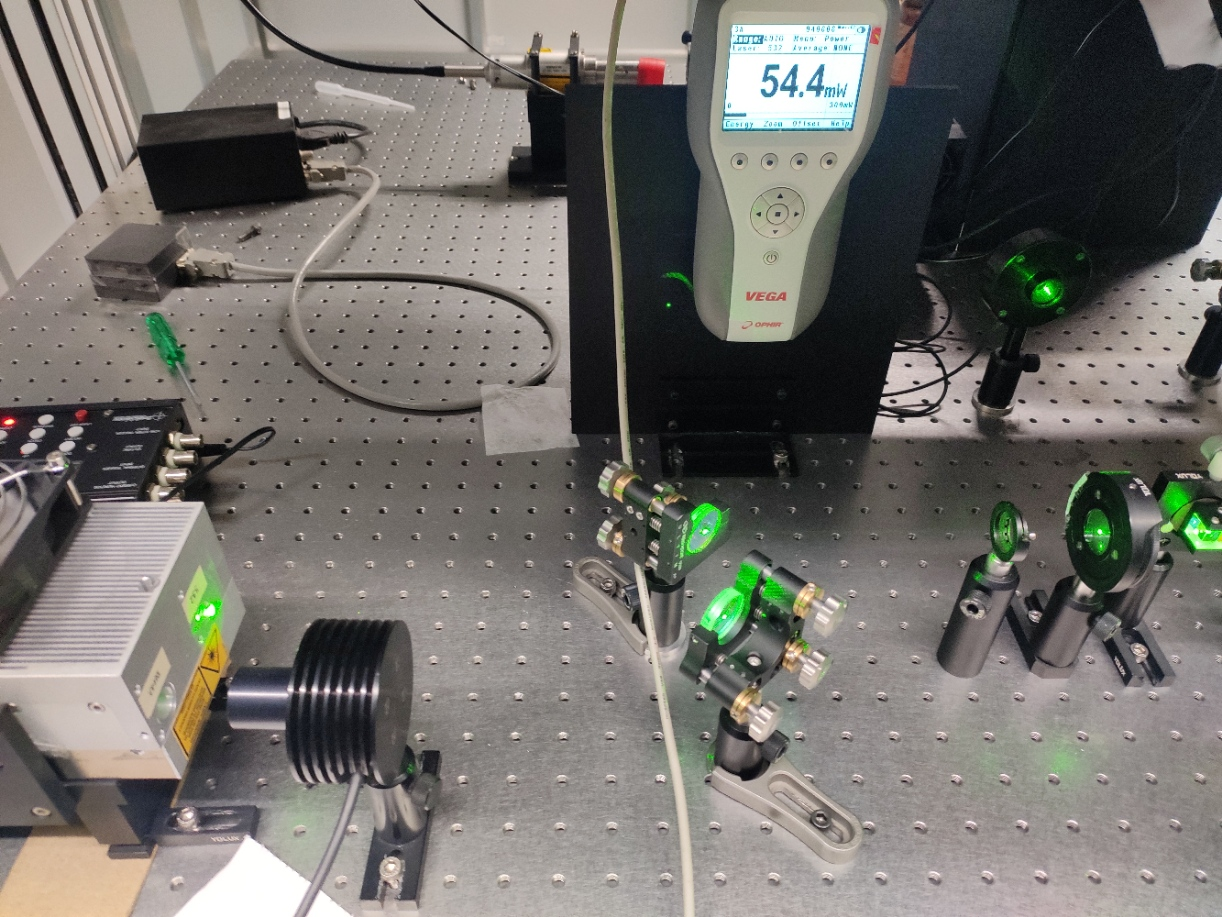
\includegraphics[width=0.9\linewidth]{images/laser.jpg}
    \caption{Experimental Setup: LASER}
    \label{fig:laser}
\end{figure}
\begin{figure}
    \centering
    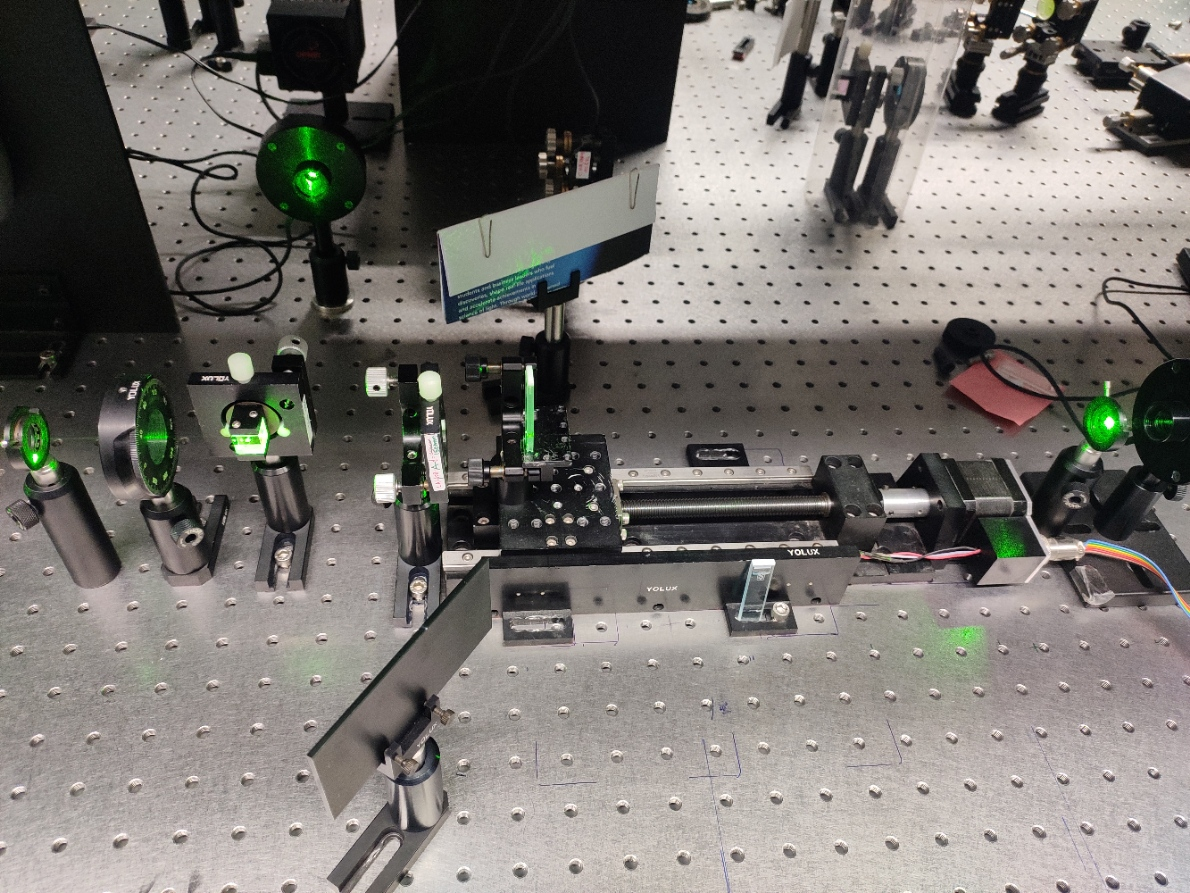
\includegraphics[width=0.9\linewidth]{images/else.jpg}
    \captionsetup{width=0.4\textwidth}
    \caption{Experimental Setup: We can observe (from the left), Aperture (A1), Half-Wave plate, Beam Splitter, Thermal Detector (TD1, near the top), Converging Lens, Translation Stage with Sample, Aperture (A2) and Thermal Detector (TD2). Multiple screens can also be seen around the setup.}
    \label{fig:else}
\end{figure}
\begin{figure}
    \centering
    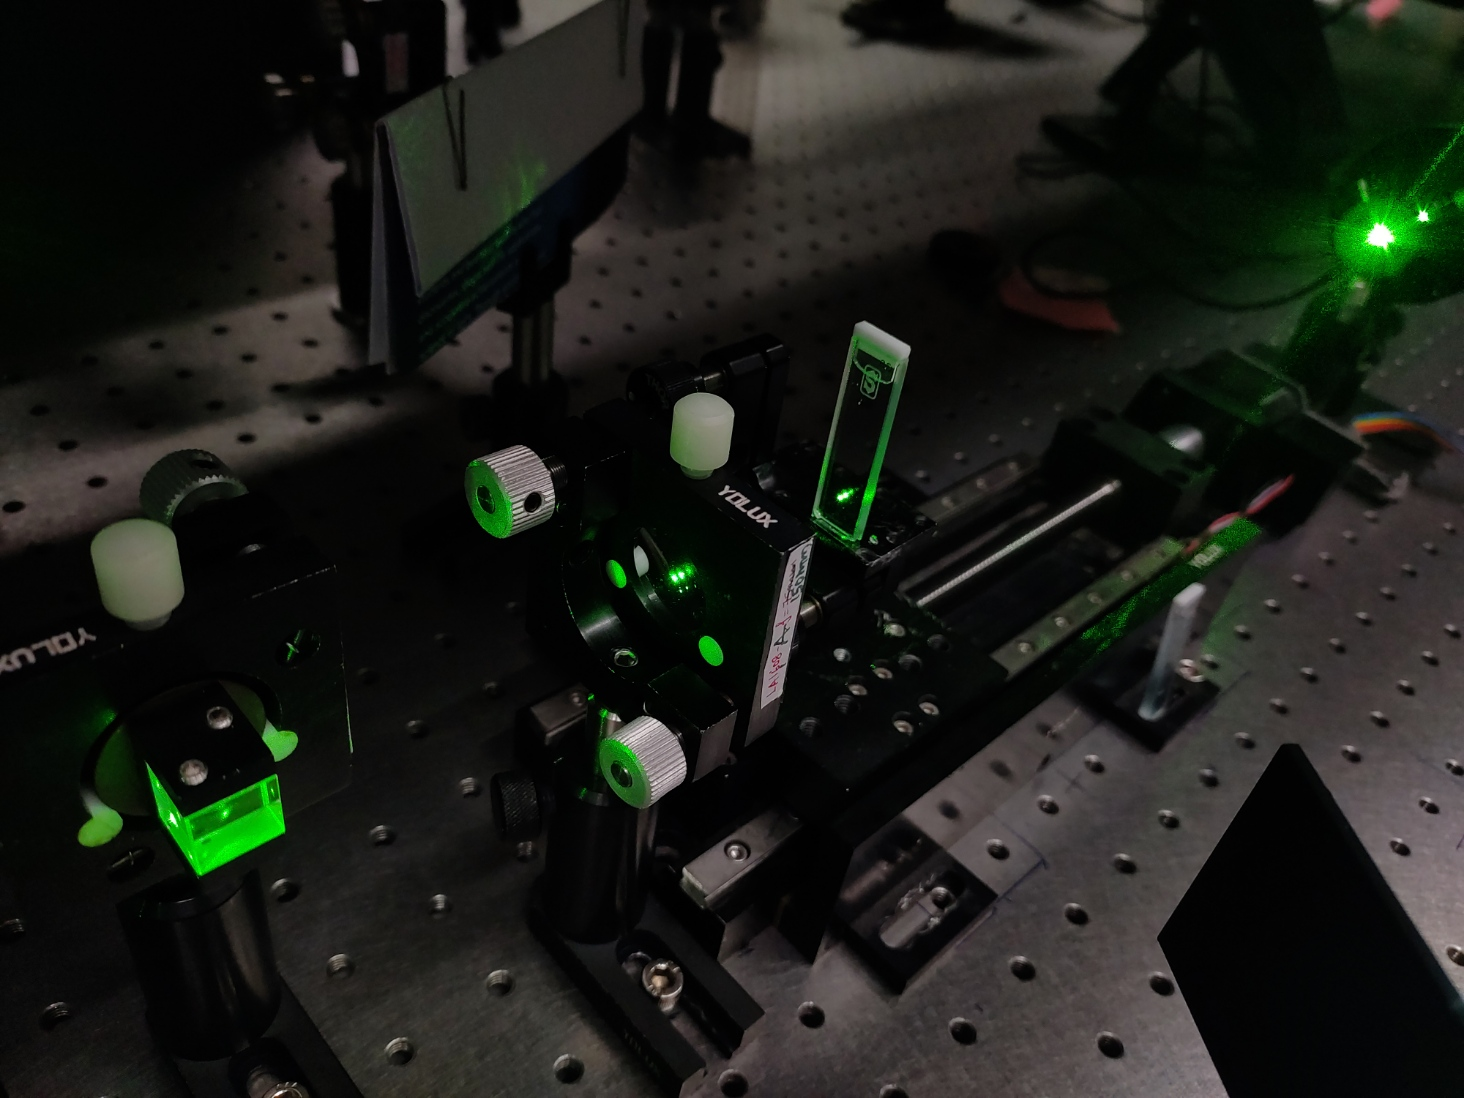
\includegraphics[width=0.9\linewidth]{images/run.jpg}
    \caption{Setup in operation}
    \label{fig:run}
\end{figure}

The schematic of the experimental setup has been presented in Fig.~\ref{fig:schem}. The LASER, used in the experiment can be seen in Fig.~\ref{fig:laser}, while the rest of the setup has been displayed in Fig.~\ref{fig:else}. Figure~\ref{fig:run} shows the setup, while a reading was being taken. In this experiment, we have taken data for 4 samples, details of which, have been provided in Table~\ref{table:sampdets} and Fig.~\ref{fig:samps}.

\begin{figure*}
\subcaptionbox{Sample 1: SKK1 (Molecular Diagram)}{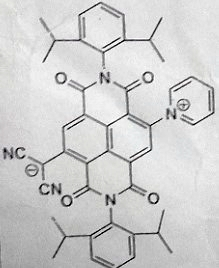
\includegraphics[width=0.22\textwidth]{images/skk1.jpg}}%
\hfill
\subcaptionbox{Sample 2: SKK2 (Molecular Diagram)}{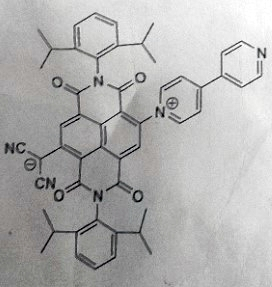
\includegraphics[width=0.22\textwidth]{images/skk2.jpg}}%
\hfill
\subcaptionbox{Sample 3: Nanorods on Tempered Glass Substrate}{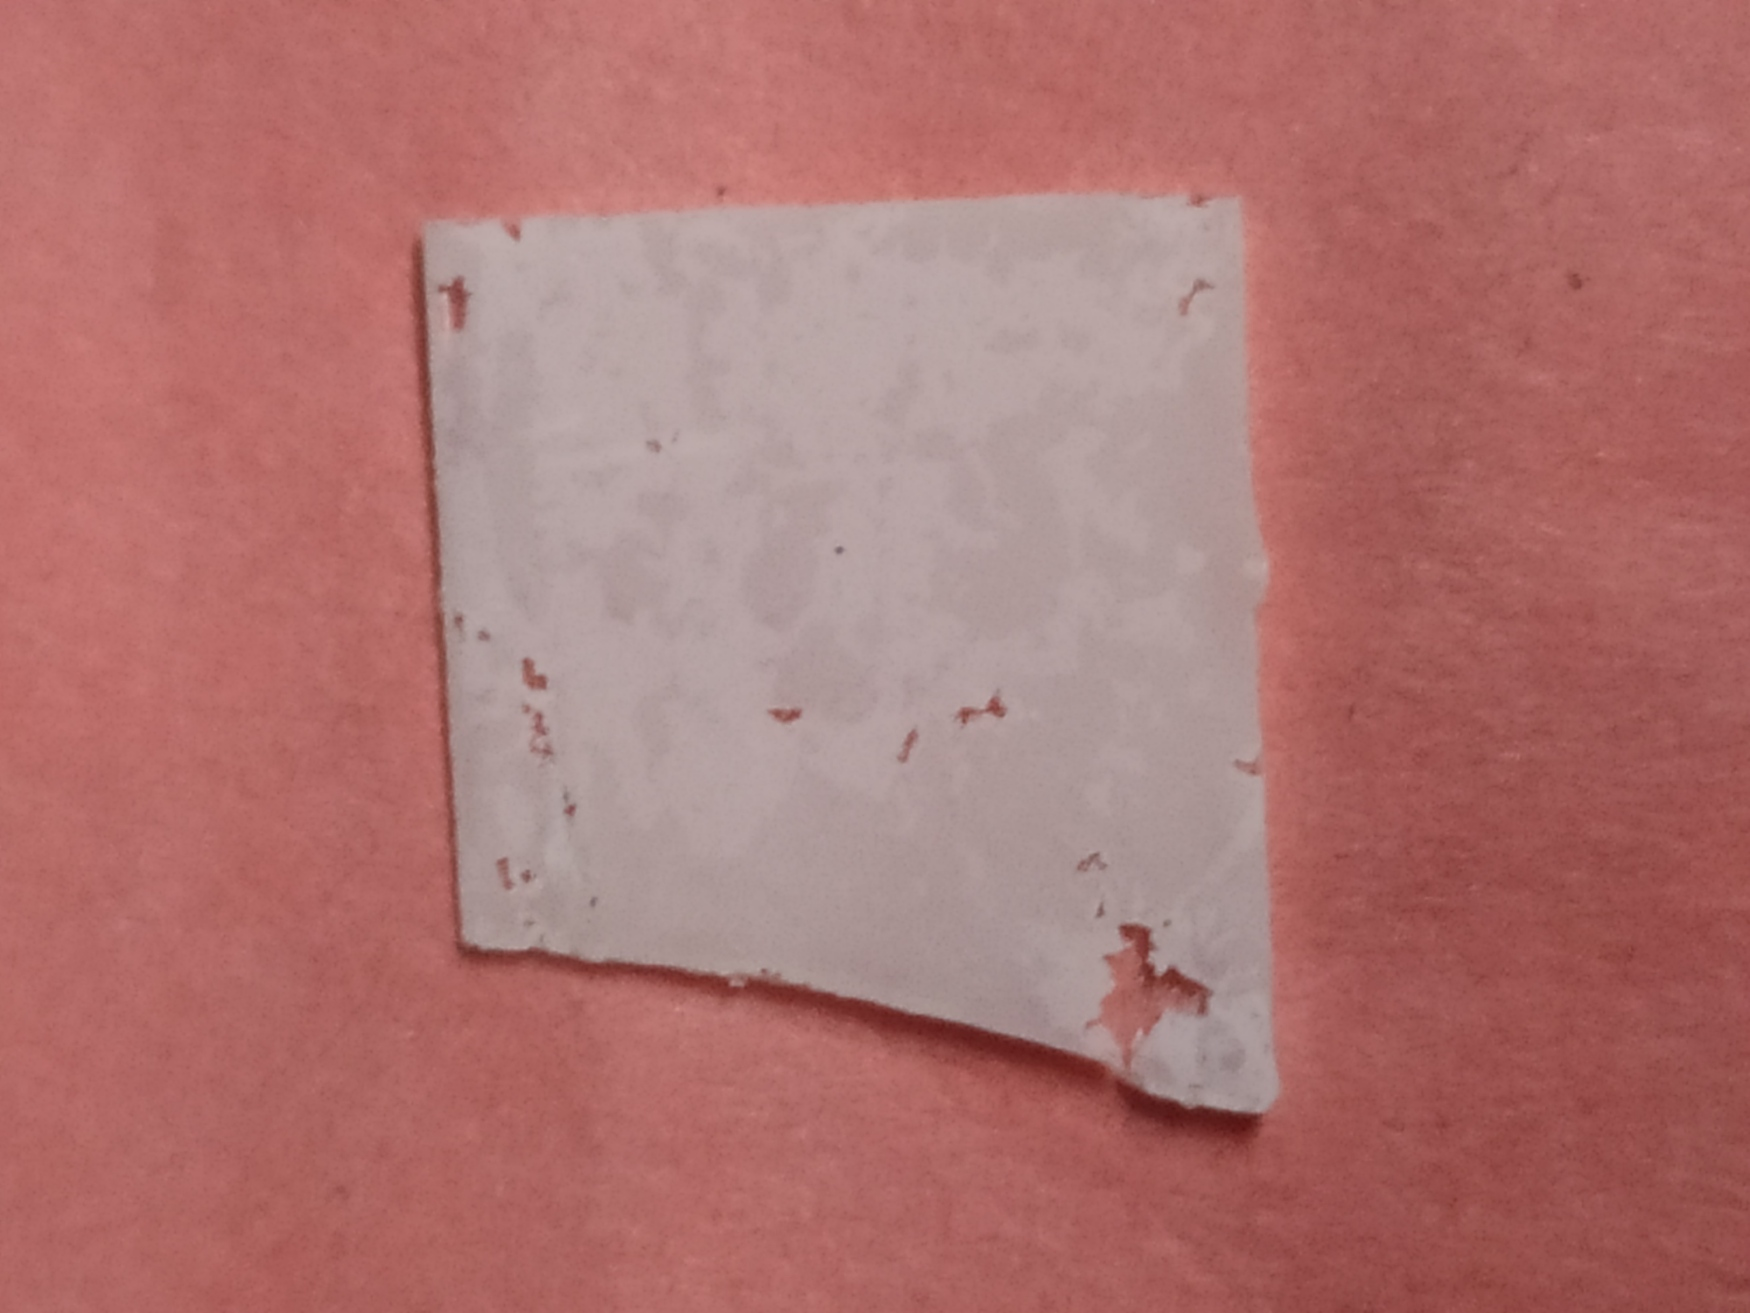
\includegraphics[width=0.24\linewidth]{images/tgls.jpg}}%
\hfill
\subcaptionbox{Sample 4: Nanorods on Standard Glass Substrate}{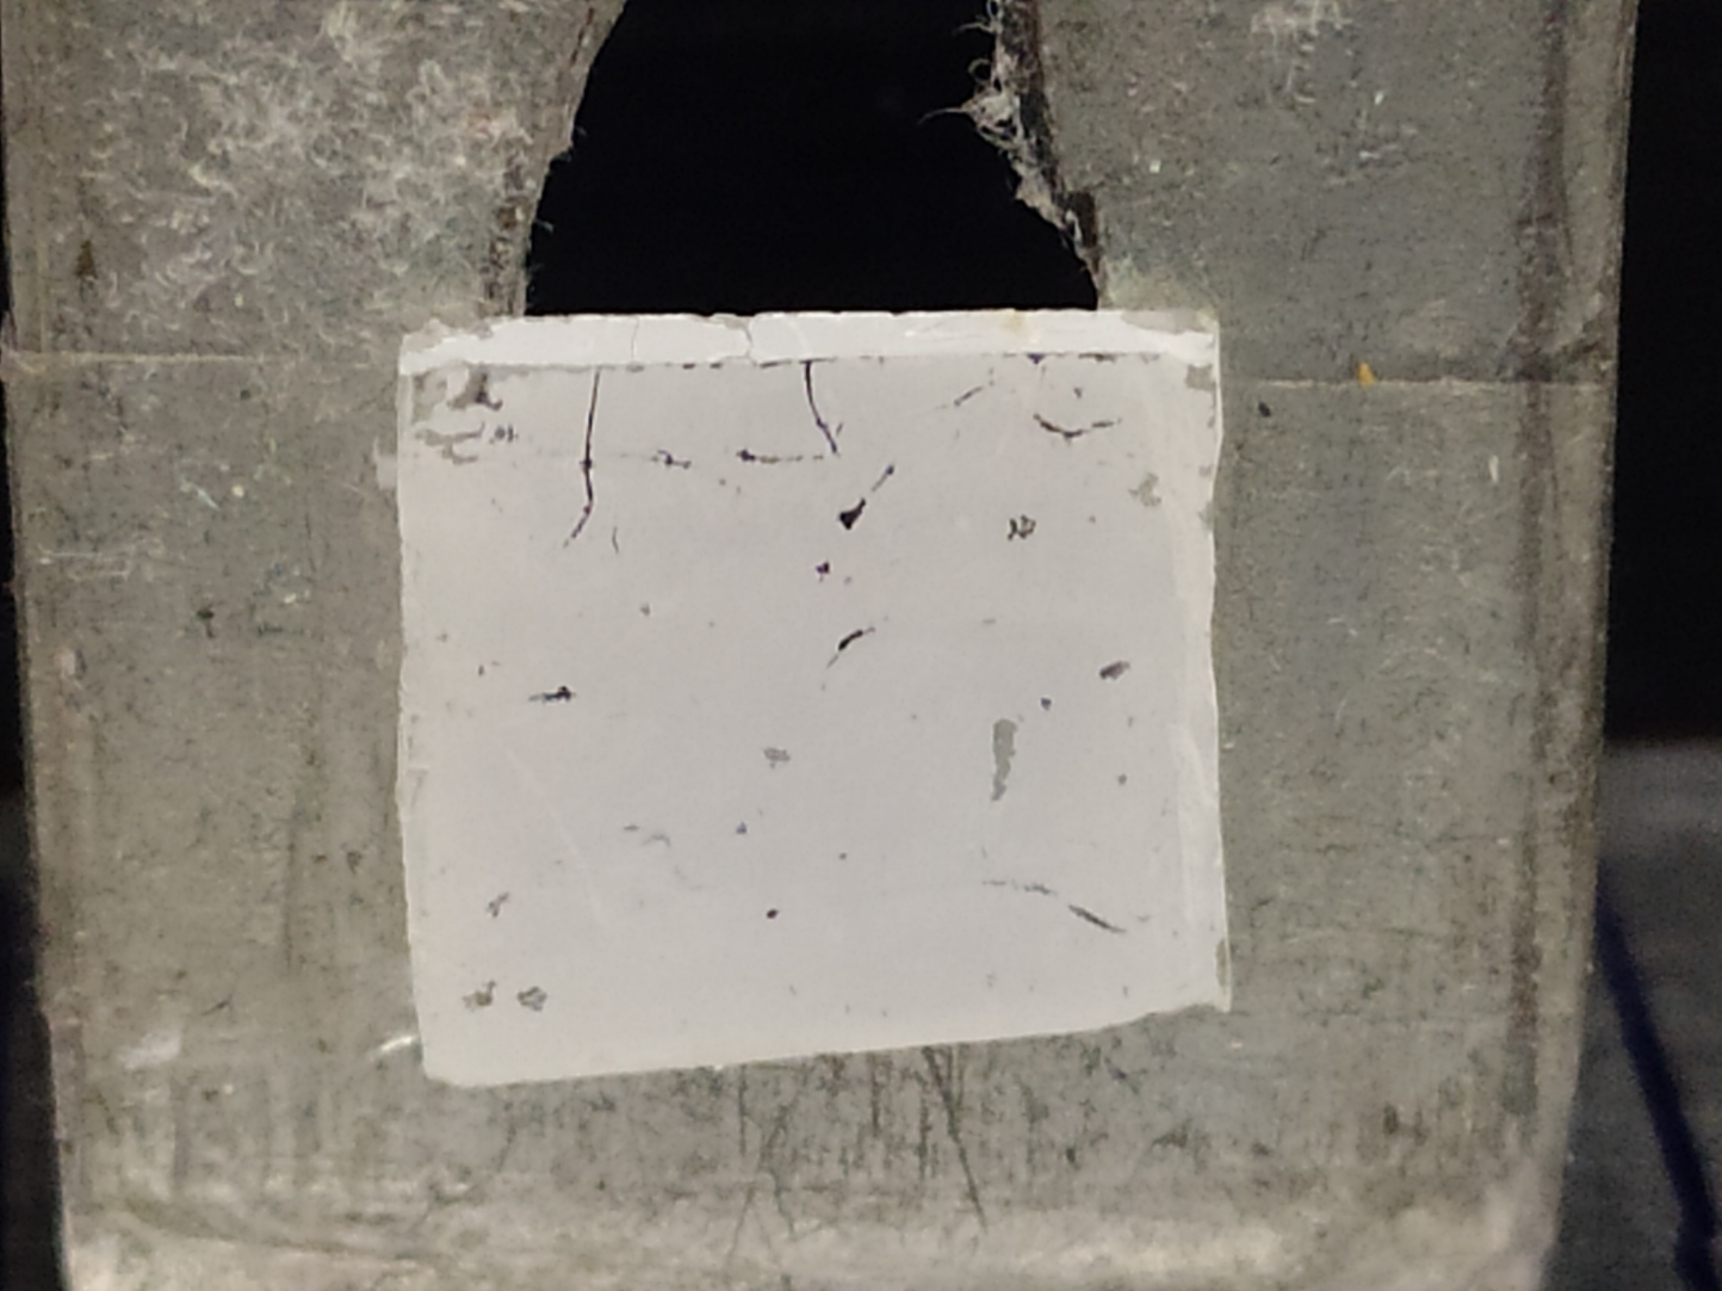
\includegraphics[width=0.24\linewidth]{images/gls.jpg}}%
\hfill
\caption{Samples used in this experiment}
\label{fig:samps}
\end{figure*}

\begin{table}
 \begin{tabular}{c|l} 
 \hline\hline
 \textbf{Sample} & \multicolumn{1}{c}{\textbf{Details}} \\
 \hline
 \multirow{5}{*}{SKK1} & Formula: $C_{46}H_{41}N_5O_4$ \\
 & Mol. Wt.: $727.848$ \\
 & Amount used: $\approx 181\:\mu g$ \\
 & Solvent used: DMSO \\
 & Molarity: $\approx5\:\mu M$ \\
 \hline
 \multirow{5}{*}[\normalbaselineskip]{SKK2} & Formula: $C_{52}H_{44}N_6O_4$ \\
 & Mol. Wt.: $804.932$ \\
 & Pre-prepared \\
 \hline
 \multirow{2}{*}{Nanorods} & Substrate: Tempered Glass \\
 & Pre-prepared \\
 \hline
 \multirow{2}{*}{Nanorods} & Substrate: Standard Glass \\
 & Pre-prepared \\
 \hline\hline
\end{tabular}
\caption{Details about the Samples}
\label{table:sampdets}
\end{table}

\subsection{\label{proc}Procedure}

The setup was first aligned with two mirrors and two apertures, with the LASER running at $40\%$ intensity and at $80\:KHz$ Repetition Rate. The mirrors were placed in a Z-Fold configuration, as can be seen in Fig.~\ref{fig:laser}. One of the apertures was placed closer to the mirrors, while the other was placed further away. Alignment was done using the pitch and yaw knobs on the mirrors. $M1$ was used to align with respect to the nearer aperture, while $M2$ was used to align with respect to the distant aperture. A simple check for alignment is that the surface of both apertures, when closed, should be illuminated uniformly. After we succeeded in aligning the LASER through $A1$ and $A2$, the Half-Wave plate, the Beam Splitter and the Lens were added and alignment was checked after each addition. At each stage, we also adjusted the mirrors to avoid back-reflection into the LASER. Then, we estimated the beam width of the LASER, using a Beam Profiler.\\

After the alignment was complete and the beam width was obtained, we prepared a sample of SKK1, as per the specifications in Table~\ref{table:sampdets}, and transferred it to a cuvette. Then, a translation stage was placed in between the Lens and $A2$ and the cuvette was attached to the stage using double-sided tape. The Thermal Detectors were also placed as shown in Fig.~\ref{fig:else}. Both, the detectors and the translation stage, were connected to a laptop. A custom-made software was used to control the stage, while \href{https://www.ophiropt.com/laser--measurement/node/11344}{StarLab 3.30} was used to record the intensity of light, falling on the detectors. Both software were acquired from the lab computer. The Repetition Rate of the LASER was set between $1\:KHz$ to $8\:KHz$ and the intensity was set to $100\%$. For each of the samples, we took various readings for both open-aperture (OA) and closed-aperture (CA) Z-Scans. In all cases, the sample was translated from the lens ($L0$) to aperture, $A2$, with the motor running at $250$ to $300$ RPM. After each reading, the sample's position was reset to near the lens. Also, for 3 of the 4 samples, we only took data for the sample itself, but for Nanorods on Tempered Glass substrate, we took Z-Scan data for tempered glass as well, so as to cancel out any ``background" contributions from the tempered glass. The plots and calculated quantities obtained from these datasets have been presented in the next section.

\section{\label{obs}Observations}
Since the data tables are large, we have uploaded the raw, as well as processed datasets on our \href{https://github.com/JeS24/z_scan}{GitHub repository}. All data has been analyzed and the plots have been produced using Jupyter notebooks (Python). We have also performed error analysis on the obtained quantities. The code for the plots as well as the error analysis, can be found in our GitHub repository. In addition to this, the intermediate calculations and fit parameters can also be found in the \href{https://github.com/JeS24/z_scan/blob/main/notebooks}{code for the respective samples} on GitHub.\\

Using the beam profiler, we have estimated the $D4\sigma$ beam width \cite{d4s} to be approximately $30\:\mu m$. However, this measurement was rough and we have taken the beam waist, and hence the Rayleigh length, to be an adjustable parameter while fitting the data. The exact values used are present in the Jupyter notebooks for the samples. The closed as well as open aperture Z-Scan traces can be found in the Appendix, near the end of this document. For the reader's convenience, we have listed direct links to all the plots in Table~\ref{table:conv}.\\

One thing to note here is that we have used slightly different normalization schemes for closed and open aperture scans. For open aperture scans, we have divided the sum of the endpoint power values by 2, while for closed aperture scans, we have taken the mean of the observed power values. This ensures $T \le 1$ for open aperture scans, while for closed aperture scans, it allows us to obtain the behaviour around $T = 1$. The normalization scheme, in code, can be found in \href{https://github.com/JeS24/z_scan/blob/main/notebooks/utils.py}{this file} on our GitHub repository.\\

The values of $n_2$ and $\beta$, along with their uncertainties, obtained from the fits, can be found in Tables~\ref{table:catab} and \ref{table:oatab}, while the $T_{p-v}$ values can be found in Table~\ref{table:catpv}. In the next section, we discuss and interpret these plots and results.

\begin{table}
 \begin{tabular}{c|c}
 \hline\hline
 \textbf{Sample} & \textbf{Figures} \\
 \hline
    SKK1 & Fig.~\ref{fig:skk1} \\
    SKK2 & Fig.~\ref{fig:skk2} \\
    Nanorods on Tempered Glass Substrate & Fig.~\ref{fig:nrtg} \\
    Nanorods on Standard Glass Substrate & Fig.~\ref{fig:nrg} \\
 \hline\hline
\end{tabular}
\captionsetup{width=0.4\textwidth}
\caption{Closed Aperture (CA) and Open Aperture (OA) Plots}
\label{table:conv}
\end{table}

\begin{table*}
 \begin{tabular}{c|r|c}
 \hline\hline
 \textbf{Sample} & \multicolumn{1}{c|}{$n_2$ ($cm^2\:W^{-1}$)}  & \textbf{$\%$-Error} \\
 \hline
 SKK1 & $(-164.9555 \pm 1.7239)\times10^{-17}$  &  $1.045\:\%$ \\
 SKK2 & $(-77.6141 \pm 1.3053)\times10^{-17}$  &  $1.682\:\%$ \\
 Nanorods on Tempered Glass Substrate & $(51.8272 \pm 1.5643)\times10^{-15}$ & $3.018\:\%$ \\
 Nanorods on Standard Glass Substrate & $(-179.5371 \pm 1.7149)\times10^{-18}$ & $0.955\:\%$ \\
 \hline\hline
\end{tabular}
\caption{Closed Aperture Z-Scan: Non-linear Refractive Index ($n_2$) for all samples}
\label{table:catab}
\end{table*}

\begin{table*}
 \begin{tabular}{c|r|c}
 \hline\hline
 \textbf{Sample} & \multicolumn{1}{c|}{$\beta$ ($\:cm\:W^{-1}$)}  & \textbf{$\%$-Error} \\
 \hline
 SKK1 & $(118.7748 \pm 1.1301)\times10^{-12}$ & $0.951\:\%$ \\
 SKK2 & $(428.4424 \pm 4.0479)\times10^{-13}$ & $0.945\:\%$ \\
 Nanorods on Tempered Glass Substrate & $(-389.1827 \pm 2.0049)\times10^{-8}$ & $0.515\:\%$ \\
 Nanorods on Standard Glass Substrate & $(-15.5681 \pm 1.0905)\times10^{-7}$ & $7.005\:\%$ \\
 \hline\hline
\end{tabular}
\caption{Open Aperture Z-Scan: Non-linear Absorption Coefficient ($\beta$) for all samples}
\label{table:oatab}
\end{table*}

\begin{table*}
 \begin{tabular}{c|c|c|c}
 \hline\hline
 \textbf{Sample} & \textbf{From Theory} & \textbf{From Fit} & \textbf{$\%$-Difference} \\
 \hline
 SKK1 & $1.2743$ & $1.2738$ & $0.0423\:\%$ \\
 SKK2 & $0.5352$ & $0.5402$ & $0.0547\:\%$ \\
 Nanorods on Tempered Glass Substrate & $0.4936$ & $0.4926$ & $0.1954\:\%$ \\
 Nanorods on Standard Glass Substrate & $0.4963$ & $0.4941$ & $0.4528\:\%$ \\
 \hline\hline
\end{tabular}
\caption{Closed Aperture Z-Scan: $T_{p-v}$ for all samples}
\label{table:catpv}
\end{table*}

\section{\label{dis}Discussion}
The nature of non-linear materials can be simplistically observed with the Single Beam Z-Scan technique. In this analysis, we have taken the closed and open aperture Z-Scans of the materials listed in Table~\ref{table:sampdets}, and have presented our results for the Non-Linear Refractive Indices ($n_2$) and the Non-Linear Absorption Coefficient ($\beta$) with the corresponding calculation done using Python. For all the cases under study, our results fall in the normally observed range of $n_2$ and $\beta$ values (Tables~\ref{table:catab} and \ref{table:oatab}). The calculated error is also quite minimal, which is also supported by the excellent match between observed and calculated $T_{p-v}$ values (Table~\ref{table:catpv}). This also implies that the working formulae (Eq.~\ref{eq:T22} and Eq.~\ref{eq:T2o}) work well in the range of phase distortions, with $\le0.5\:\%$ difference for $\Delta\Phi_0 \le \pi$, in this experiment. We have also tried using a slightly modified 2-parameter function to fit the closed aperture scans, as given in Nguyen et al \cite{nguyen}, but in our case, the function obtained by Sheikh-Bahae et al \cite{bahae} gives slightly better results for all samples. As for the plots themselves, we have observed usual third order non-linear behaviour for SKK1 and SKK2, but with the Nanorods sample on both substrates, we have also observed Saturable Absorption (Figures~\ref{fig:nrtg} and \ref{fig:nrg}). Another thing to note is that, for the Nanorods samples, the vastly dissimilar $n_2$ and $\beta$ values imply that the substrates seem to affect the optical properties of the samples. This could also be a consequence of the fabrication process.\\

From the Jupyter notebook for Nanorods on Tempered Glass, we note that, subtracting the background contributions from tempered glass does help in smoothing out the data. Moreover, we have tested whether rescaling the closed aperture scan data with the open aperture scan data is helpful in emphasizing the closed aperture plot. We find that, it is indeed useful in cases, where the data does not show the expected behaviour. This can be seen in the Jupyter Notebook \href{https://github.com/JeS24/z_scan/blob/main/notebooks/NanoRods\%20on\%20TG\%20-\%20Rescaling.ipynb}{here}.\\

Apart from these main results, we also tried tweaking certain environmental or setup parameters, such as the RPM of the stepper motor in the translation stage, as well as the intensity of the LASER light. In the first case, we could only observe slightly irregular plots, which correlate with the sampling rate of the thermal detectors and can be dismissed as experimental noise, while in the latter case, we observed different outcomes with different materials. For SKK1 and SKK2, increasing the intensity only ``smoothed" the plots, which is as expected. But with Nanorods on either substrates, sign inversion seemed to take place at very high intensities. This can be explained by considering a transition from Saturable Absorption to Reverse Saturable Absorption.\\

Also, while the fitting function does seem to give us good results, the fitted curves do not seem to match up with the experimental data in some of the plots. This apparent discrepancy can be explained by the fact that we have tried to adjust the fit parameters (such as Beam Width) so as to give us the best possible matching between the peaks of the experimental data and the fitted curve. This premise is upheld by the nice $T_{p-v}$ values in Table~\ref{table:catpv}. As for the rest of the plot, the fit seems to diverge from the data in some cases. This can be attributed to several factors such as noise from the translation stage or fluctuations in LASER intensity which can lead to contributions from higher order and thermal effects. But the most important factor, in all cases, appears to be the average LASER power at which the data was taken. In all cases, where the experimental and fitted curves seem to diverge, the average LASER power is small, almost at the least count of the thermal detectors, while for cases, where the LASER power could be much higher, we have obtained smoother plots. The actual power values can be found in the raw data files or the Jupyter notebooks, present in the GitHub repository. Another thing to note is the small blip in the open aperture Z-Scan trace for SKK2 (Fig.~\ref{fig:skk2}), that indicates small contributions from higher order non-linearities. Opposite contributions from the competing effects of Two-photon Absorption (2PA) and Saturable Absorption (SA) could also be a factor, as discussed in \cite{wang} and \cite{mori}.\\

In conclusion, we have explored and applied the Z-Scan technique and the theory of third order non-linear optics in this experiment. We have worked with 4 samples and studied their Z-Scan behaviours and calculated their corresponding non-linear properties. In the next subsections, we discuss a frustrating issue with the setup, and some future extensions to this experiment.


\subsection{\label{issues}Setup: Issues \& Improvements}

A rather frustrating issue with the setup, that is worth mentioning, is the motorized translation stage, specifically its unstable control software. During the experiment, the control software would become unresponsive and the stage would abruptly stop for several seconds, leading to loss of experimental data for several runs. Moreover, the number of steps itself does not directly correlate with the actual length traversed, for a constant RPM, thereby adding some uncertainty to the translation length of the sample. A more functional translation stage would certainly help take some of this frustration away and make the experiment straightforward.\\

While this (admittedly minor) issue does necessitate some modifications to the setup, we can also enhance the experiment itself with some interesting extensions. We discuss these in the next subsection. 

\subsection{\label{future}Notes \& Future Extensions}

In this experiment, we have focused exclusively on the third order non-linearities, but as we can discern from the plots, in some cases, higher order non-linearities also play a role. Therefore, we can broaden the scope of this experiment by taking into account higher order contributions, specifically the fifth order. A good theoretical starting point for this is the article by Gu et al \cite{gu}.\\

We can also try the 3-Photon Absorption (3PA) Equation as the fitting function to help explain the blip in the open aperture Z-Scan trace for SKK2. A useful resource for this is Rangel-Rojo et al \cite{3pa}, wherein the authors discuss simultaneous 2PA and 3PA in Polydiacetylene Zwitterions. This relates to the zwitterionic structure of SKK2 and can perhaps help explain the slight deviation.\\

As mentioned before, at reasonably high intensities (such that the material itself is not damaged), the Nanorods samples exhibit sign-switching in the open aperture trace. This can lead to another extension to this experiment in the form of study of the optical properties of such materials. Srinivas et al \cite{srini} and Yüksek et al \cite{yuk} have worked on similar materials in their respective works.\\

There are more topics of interest in this domain, but all the aforementioned extensions of this experiment have the advantage of keeping the setup unmodified.

\subsection{\label{precautions}Precautions}
We have listed some of the precautions taken during the experiment below:
\begin{enumerate}
    \item The setup was aligned properly before the data was taken, in order to minimize deviations from the $z-$line.
    \item The samples were placed symmetrically with respect to the LASER beam, in order to avoid edge effects.
    \item Since we were working with a high power LASER, all precautions were taken to ensure that no eye or skin damage would occur. We used the polarizer or the LASER control unit to safely lower the LASER intensity, or screens to completely block the light, when adjusting the setup.
    \item Clean gloves were worn while handling samples, so as to avoid contaminating them and hence the scan data.
    \item The cuvettes for the liquid samples were cleaned with organic solvents, before the samples were transferred into them. This was done to minimize the effect of the material of the cuvette or dust, on the scan data.
    \item For the Nanorods samples on substrates, the layering of the material was uneven (Fig.~\ref{fig:samps}). In this case, we ensured that the LASER light passed through the smoothest area on the sample.
    \item In all cases, the LASER was blocked after every few runs, in order to cool off the sample, as thermal instabilities can affect the scans.
\end{enumerate}

\begin{acknowledgments}
We would like to express our gratitude towards Mr. Soumik Nandi, Ms. Anupa Kumari and Dr. Ritwik Das for insightful discussions on various aspects of this experiment.
\end{acknowledgments}


% The \nocite command causes all entries in a bibliography to be printed out
% whether or not they are actually referenced in the text. This is appropriate
% for the sample file to show the different styles of references, but authors
% most likely will not want to use it.
% \nocite{*}
\bibliography{main}% Produces the bibliography via BibTeX.
\pagebreak
\newpage
\onecolumngrid
\appendix
\newpage
\section*{Appendix: Z-Scan Traces}
\label{app:plots}

\begin{figure*}[h]
\subcaptionbox{Closed Aperture Curve}{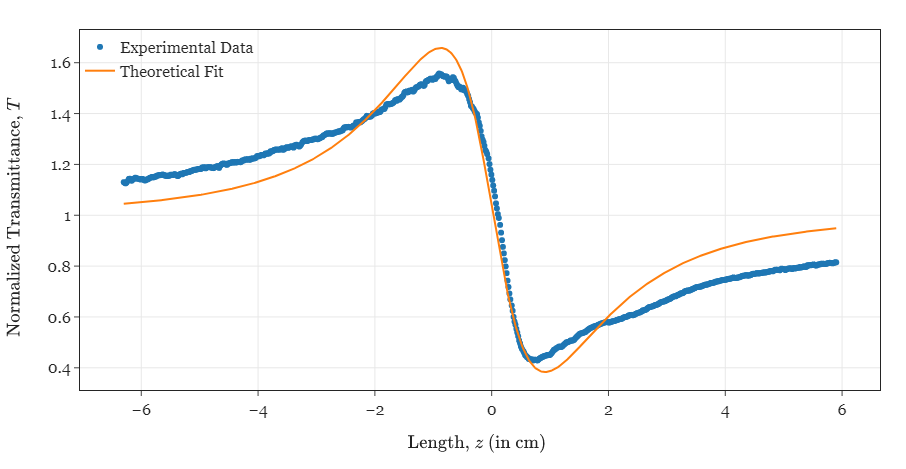
\includegraphics[width=\textwidth]{images/skk1_ca.png}}%
\hfill
\subcaptionbox{Open Aperture Curve}{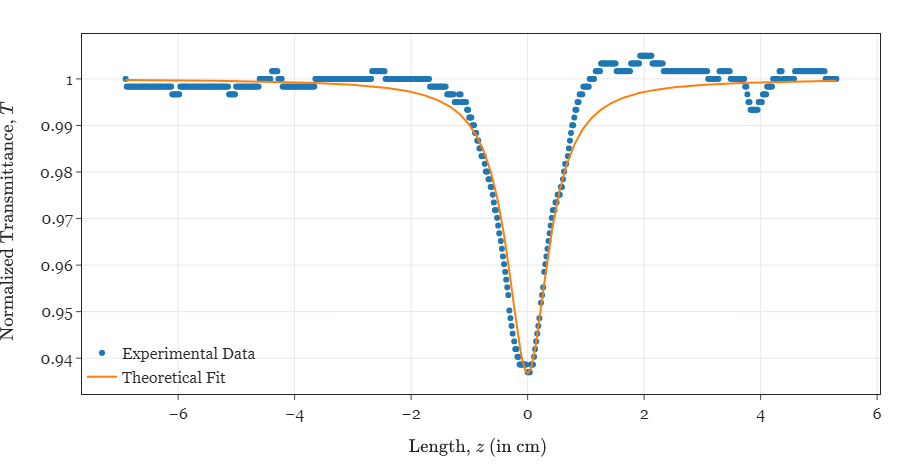
\includegraphics[width=\textwidth]{images/skk1_oa.png}}%
\hfill
\caption{Sample 1: SKK1}
\label{fig:skk1}
\end{figure*}

\begin{figure*}[h]
\subcaptionbox{Closed Aperture Curve}{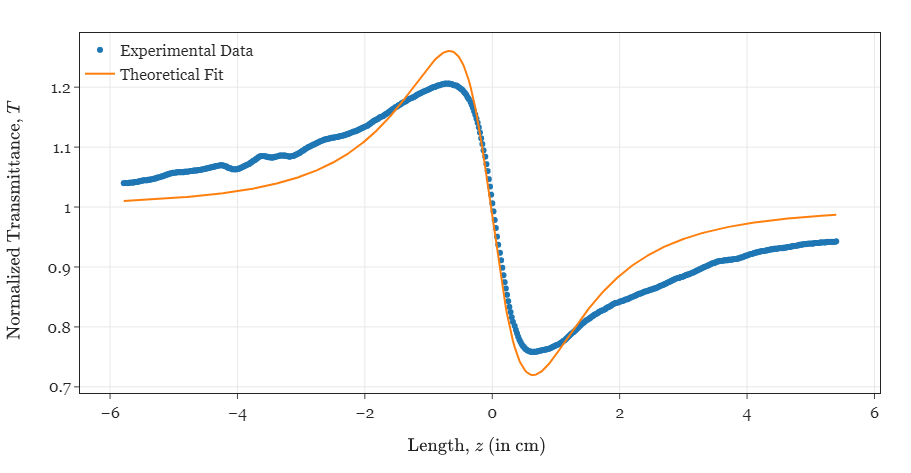
\includegraphics[width=\textwidth]{images/skk2_ca.png}}%
\hfill
\subcaptionbox{Open Aperture Curve}{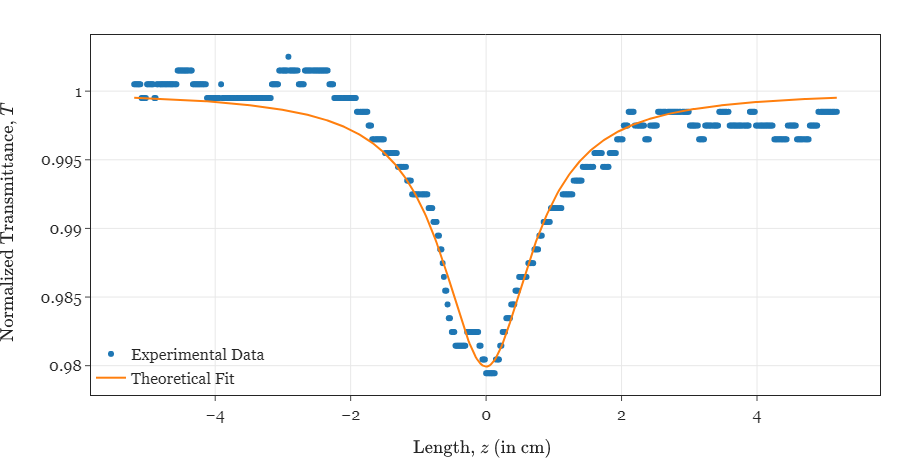
\includegraphics[width=\textwidth]{images/skk2_oa.png}}%
\hfill
\caption{Sample 2: SKK2}
\label{fig:skk2}
\end{figure*}

\begin{figure*}[h]
\subcaptionbox{Closed Aperture Curve}{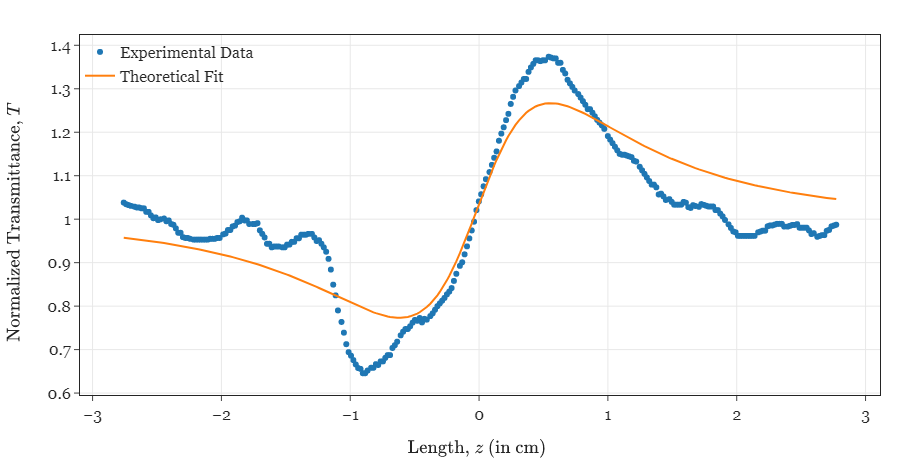
\includegraphics[width=\textwidth]{images/nrtg_ca.png}}%
\hfill
\subcaptionbox{Open Aperture Curve}{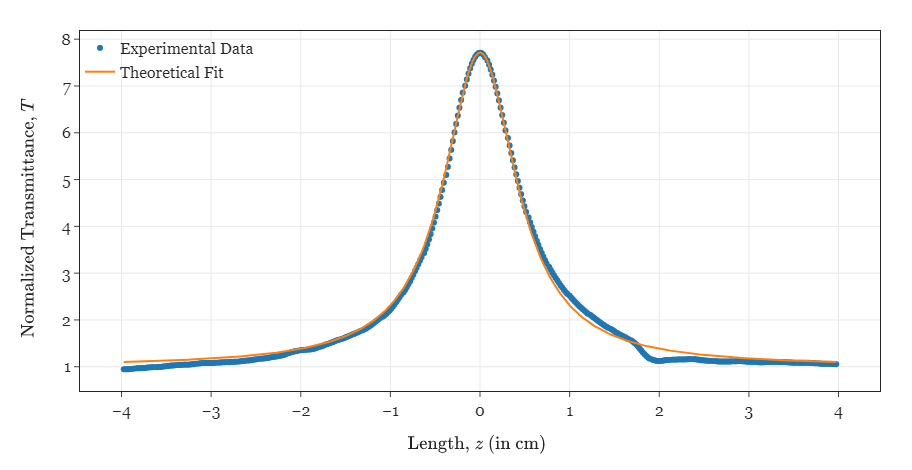
\includegraphics[width=\textwidth]{images/nrtg_oa.png}}%
\hfill
\caption{Sample 3: Nanorods on Tempered Glass Substrate}
\label{fig:nrtg}
\end{figure*}

\begin{figure*}[h]
\subcaptionbox{Closed Aperture Curve}{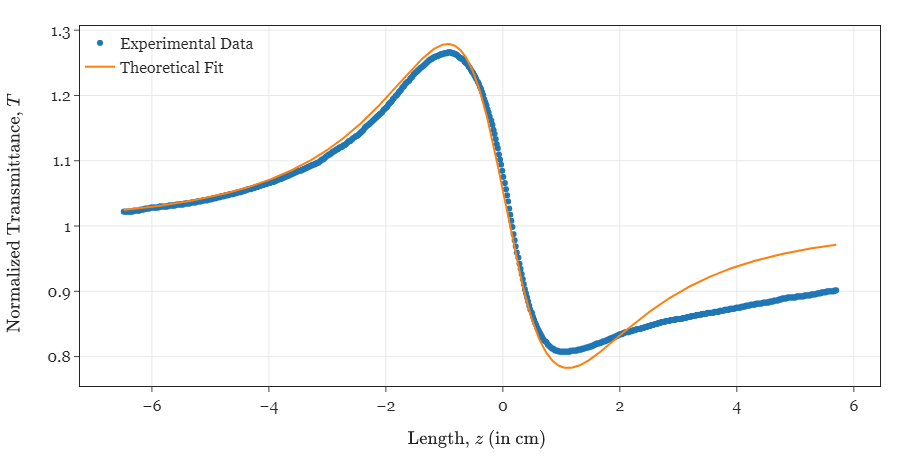
\includegraphics[width=\textwidth]{images/nrg_ca.png}}%
\hfill
\subcaptionbox{Open Aperture Curve}{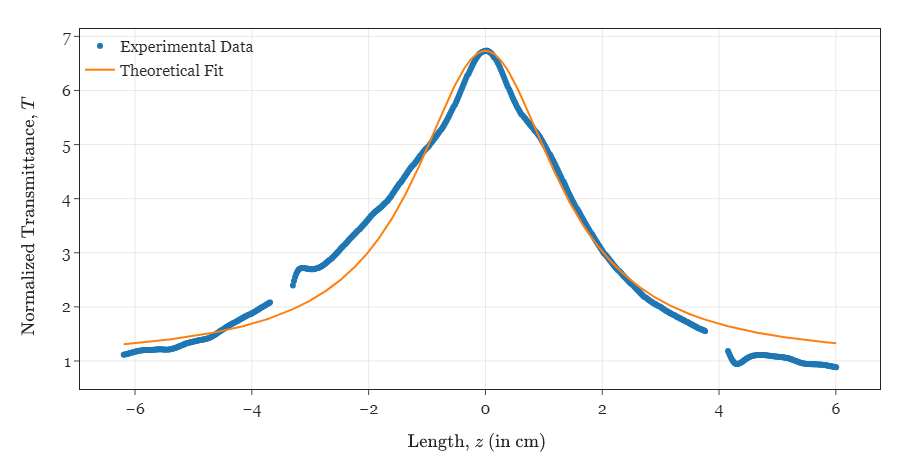
\includegraphics[width=\textwidth]{images/nrg_oa.png}}%
\hfill
\caption{Sample 4: Nanorods on Standard Glass Substrate}
\label{fig:nrg}
\end{figure*}

\end{document}
